\documentclass[margin=6pt]{standalone}
\usepackage{tikz}
\usepackage{pgfplots}
\pgfplotsset{compat = 1.18}
\tikzset{
    anc/.style ={circle,inner sep =2pt,fill=red,
    pin ={#1}}
}
\def\fun#1#2{node [anc=#1:{#2}] at (#2) {}}

\begin{document}
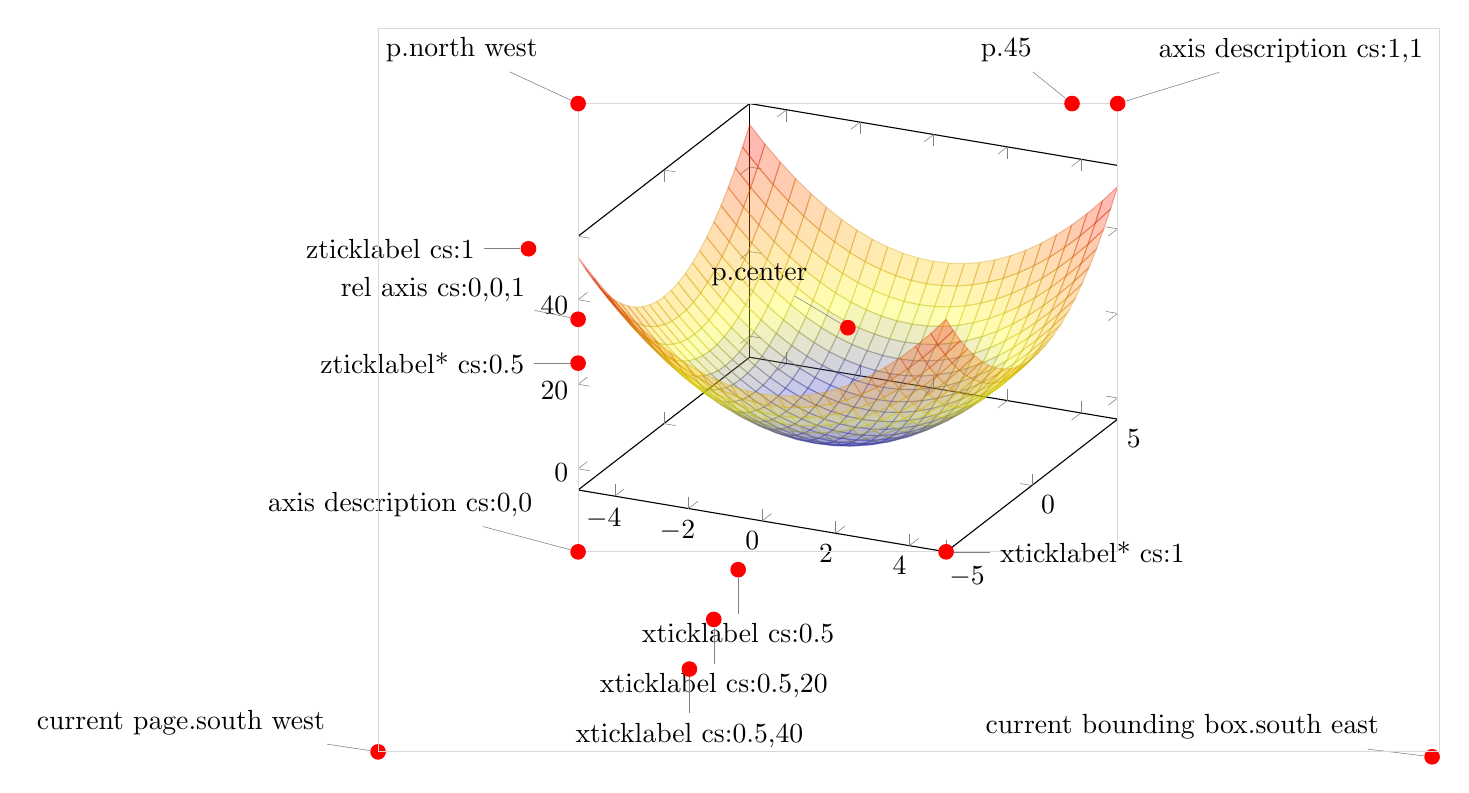
\begin{tikzpicture} 
\begin{axis}[name = p,  clip = false]
\addplot3 [surf,opacity = 0.3] {x^2+y^2};

% 坐标系中边框
\draw [black!15] (axis description cs:0,0) rectangle (axis description cs:1,1);
\path 
    \fun{45}{axis description cs:1,1}
    \fun{145}{axis description cs:0,0} 
    \fun{-90}{xticklabel cs:0.5}
    \fun{-90}{xticklabel cs:0.5,20}
    \fun{-90}{xticklabel cs:0.5,40}
    \fun{0}{xticklabel* cs:1}
    \fun{180}{zticklabel cs:1}
    \fun{180}{zticklabel* cs:0.5} 
;
\end{axis}

\path 
    \fun{170}{current bounding box.south east}
    \fun{134}{p.north west}
    \fun{134}{p.center}
    \fun{134}{p.45}
    \fun{170}{current page.south west}
    \fun{170}{rel axis cs:0,0,1}
;
% 坐标系中边框
\draw [black!15] (current page.south west) rectangle (current bounding box.north east);


\end{tikzpicture}
\end{document}